\documentclass[a4paper,12pt]{article}

\usepackage{gensymb}
\usepackage{graphicx}

\begin{document}
    \section*{Dynamics}
        \subsection*{Exercise \#1}
            Consider the wheel shown in the picture, acted on by two forces. What
            magnitude of the force F2 will be required for the wheel to be in rotational
            equilibrium?

            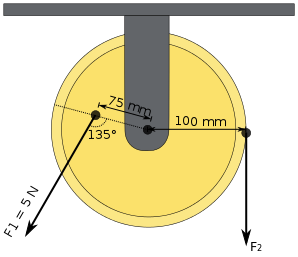
\includegraphics{img/torque-angular-momentum-ex1.png}

            \textbf{Solution}:
                
            The wheel will be in rotational equilibrium if the sum of torques is 0:

            \begin{center}$M_1 + M_2 = 0$.\end{center}

            The first torque is positive, the second one is negative. So:

            \begin{center}
                $F_1 d_1 sin(\alpha) - F_2 d_2 sin(\beta) = 0$;
                
                $F_2 = {F_1 d_1 sin(\alpha) \over d_2 sin(\beta)}$;

                $F_2 = {5N \times 75mm \times sin(135 \degree) \over 100mm} \approx 2.65N$;
            \end{center}

            \textbf{Answer}: $F_2 = 2.65N$

\end{document}
